\newcommand{\svcourse}{CST Part IA: Software Engineering and Security}
\newcommand{\svnumber}{1}
\newcommand{\svvenue}{Microsoft Teams}
\newcommand{\svdate}{2022-05-11}
\newcommand{\svtime}{15:00}
\newcommand{\svuploadkey}{CBd13xmL7PC1zqhNIoLdTiYUBnxZhzRAtJxv/ytRdM1r7qIfwMsxeVwM/pPcIo8l}

\newcommand{\svrname}{Dr Sam Ainsworth}
\newcommand{\jkfside}{oneside}
\newcommand{\jkfhanded}{yes}

\newcommand{\studentname}{Harry Langford}
\newcommand{\studentemail}{hjel2@cam.ac.uk}


\documentclass[10pt,\jkfside,a4paper]{article}
\usepackage{graphicx}

% DO NOT add \usepackage commands here.  Place any custom commands
% into your SV work files.  Anything in the template directory is
% likely to be overwritten!

\usepackage{fancyhdr}

\usepackage{lastpage}       % ``n of m'' page numbering
\usepackage{lscape}         % Makes landscape easier

\usepackage{verbatim}       % Verbatim blocks
\usepackage{listings}       % Source code listings
\usepackage{graphicx}
\usepackage{float}
\usepackage{epsfig}         % Embed encapsulated postscript
\usepackage{array}          % Array environment
\usepackage{qrcode}         % QR codes
\usepackage{enumitem}       % Required by Tom Johnson's exam question header

\usepackage{hhline}         % Horizontal lines in tables
\usepackage{siunitx}        % Correct spacing of units
\usepackage{amsmath}        % American Mathematical Society
\usepackage{amssymb}        % Maths symbols
\usepackage{amsthm}         % Theorems

\usepackage{ifthen}         % Conditional processing in tex

\usepackage[top=3cm,
            bottom=3cm,
            inner=2cm,
            outer=5cm]{geometry}

% PDF metadata + URL formatting
\usepackage[
            pdfauthor={\studentname},
            pdftitle={\svcourse, SV \svnumber},
            pdfsubject={},
            pdfkeywords={9d2547b00aba40b58fa0378774f72ee6},
            pdfproducer={},
            pdfcreator={},
            hidelinks]{hyperref}

\renewcommand{\headrulewidth}{0.4pt}
\renewcommand{\footrulewidth}{0.4pt}
\fancyheadoffset[LO,LE,RO,RE]{0pt}
\fancyfootoffset[LO,LE,RO,RE]{0pt}
\pagestyle{fancy}
\fancyhead{}
\fancyhead[LO,RE]{{\bfseries \studentname}\\\studentemail}
\fancyhead[RO,LE]{{\bfseries \svcourse, SV~\svnumber}\\\svdate\ \svtime, \svvenue}
\fancyfoot{}
\fancyfoot[LO,RE]{For: \svrname}
\fancyfoot[RO,LE]{\today\hspace{1cm}\thepage\ / \pageref{LastPage}}
\fancyfoot[C]{\qrcode[height=0.8cm]{\svuploadkey}}
\setlength{\headheight}{22.55pt}


\ifthenelse{\equal{\jkfside}{oneside}}{

 \ifthenelse{\equal{\jkfhanded}{left}}{
  % 1. Left-handed marker, one-sided printing or e-marking, use oneside and...
  \evensidemargin=\oddsidemargin
  \oddsidemargin=73pt
  \setlength{\marginparwidth}{111pt}
  \setlength{\marginparsep}{-\marginparsep}
  \addtolength{\marginparsep}{-\textwidth}
  \addtolength{\marginparsep}{-\marginparwidth}
 }{
  % 2. Right-handed marker, one-sided printing or e-marking, use oneside.
  \setlength{\marginparwidth}{111pt}
 }

}{
 % 3. Alternating margins, two-sided printing, use twoside.
}


\setlength{\parindent}{0em}
\addtolength{\parskip}{1ex}

% Exam question headings, labels and sensible layout (courtesy of Tom Johnson)
\setlist{parsep=\parskip, listparindent=\parindent}
\newcommand{\examhead}[3]{\section{#1 Paper #2 Question #3}}
\newenvironment{examquestion}[3]{
\examhead{#1}{#2}{#3}\setlist[enumerate, 1]{label=(\alph*)}\setlist[enumerate, 2]{label=(\roman*)}
\marginpar{\href{https://www.cl.cam.ac.uk/teaching/exams/pastpapers/y#1p#2q#3.pdf}{\qrcode{https://www.cl.cam.ac.uk/teaching/exams/pastpapers/y#1p#2q#3.pdf}}}
\marginpar{\footnotesize \href{https://www.cl.cam.ac.uk/teaching/exams/pastpapers/y#1p#2q#3.pdf}{https://www.cl.cam.ac.uk/\\teaching/exams/pastpapers/\\y#1p#2q#3.pdf}}
}{}


\begin{document}

\section{Thought Experiment}

Find an example of an interface from each of the waves of HCI (ideally with
similar areas of application). Next, identify the target users and their
characteristics for each. What fundamental changes appeared about the user
personas? Are there any patterns you could identify in each wave? What could
be the next wave of HCI? (Feel free to skip answering the last one, but its
worth thinking about. Hint: look at trends in hardware and software,
then think about societal trends surrounding the use of technology. What do
people like/dislike? What do companies/providers focus on/fight?)

I will discuss interfaces relating to how people communicated over the
internet. Firstly, I will discuss old-fashioned email -- non-standard email
which users manually configured. In relation to second-wave I'll discuss the
modernisation of email in the wake of papers such as ``why Johnny can't
encrypt'', which arose after behavioural scientists realised most people
weren't using email correctly. Finally, I'll discuss modern
communication apps (social media) which people use to communicate now. This
leads onto my hypothesis for fourth-wave HCI\@.

\begin{itemize}

\item In first-wave HCI, systems were designed by experts for efficient
completion of well-designed tasks by a small subset of target users. The 
user-interface was designed as a separate system (if at all) sometimes as an 
afterthought.

First Wave HCI is characterised by systems which are extremely efficient for
experts doing tasks the designers expected them to do, but very difficult
for amateur or casual users or anyone trying to do anything unconventional.
UIs almost always had little-to-no visual appeal -- that wasn't their 
intention.

Consider this example of an email UI from 1984

\begin{center}
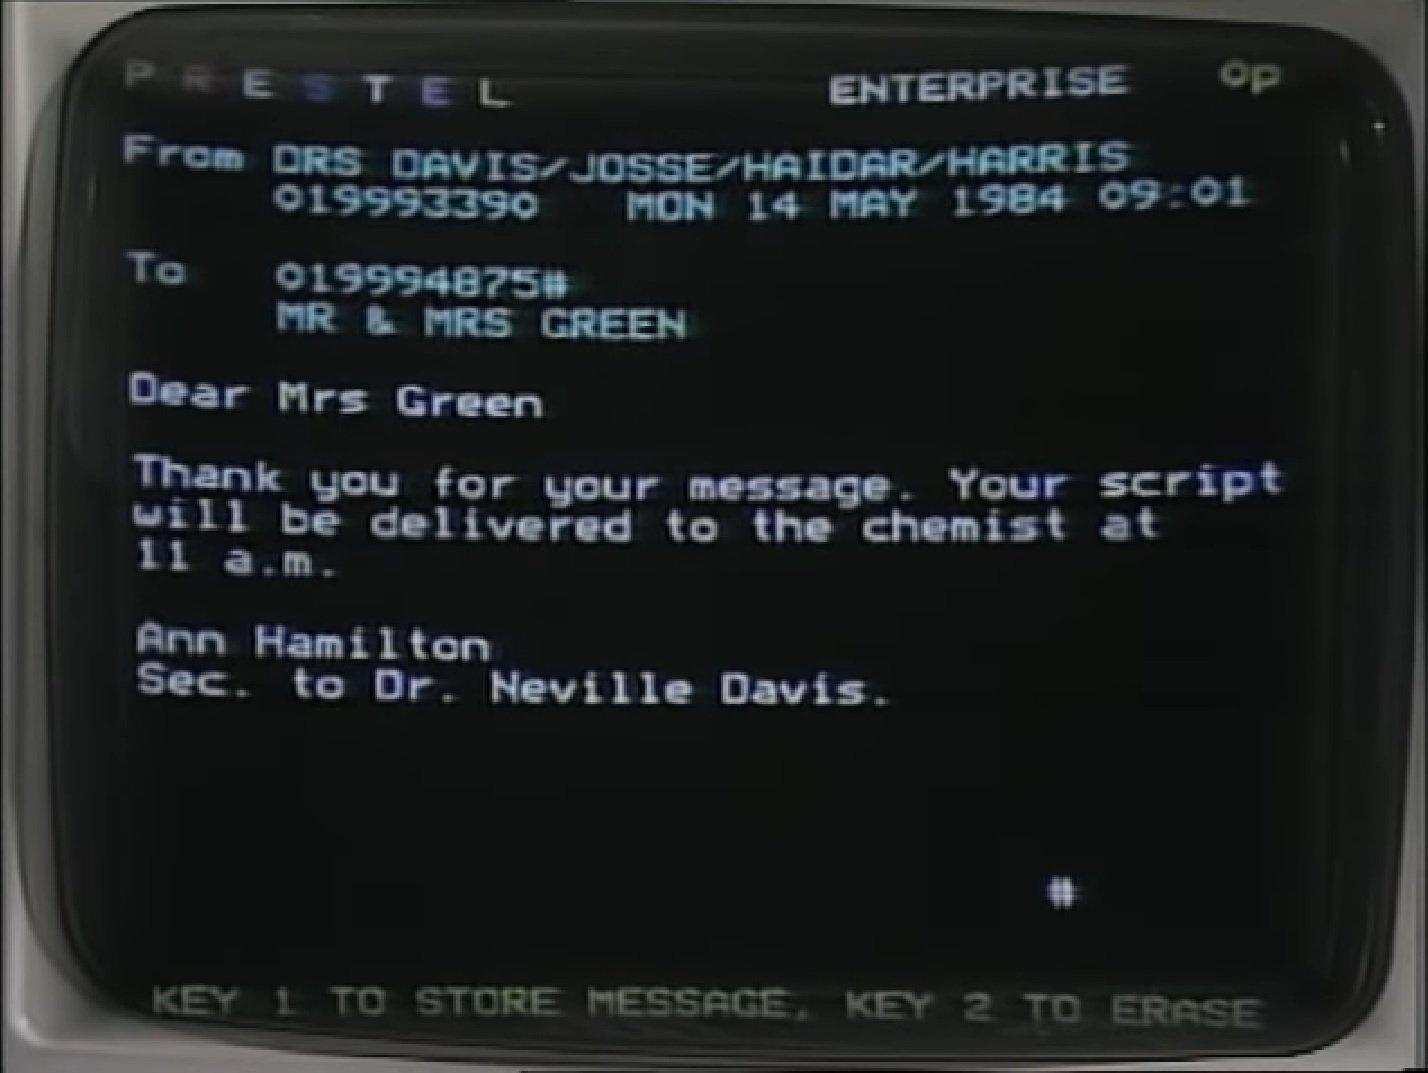
\includegraphics[width=0.4\textwidth]{1984email}
\end{center}

The interface contains all the information required to send and receive
textual information over the phone line. However, if you wanted to encrypt 
an email or send an image, the system would be unable to easily support this. 
Furthermore, to send an email, users must use the command-line and do 
extensive manual configuration.

\item In second-wave HCI, designers realised tasks weren't always 
well-defined and users weren't always who the software developers expected
they would be. This led to the ideas of social science and psychology being
incorporated into user-interfaces. Designers would visit, watch and talk
to the target users of their systems. This led to surprising revelations,
for example: not everyone can use the command line and businesses want to
encrypt data.

Second-wave HCI is characterised by design ethnography -- systems aligned
well with what users wanted them to do. They often supported more complex
operations and made goal-oriented searches easy.

Consider this email interface from 2004 -- towards the end of the
second-wave of HCI:

\begin{center}
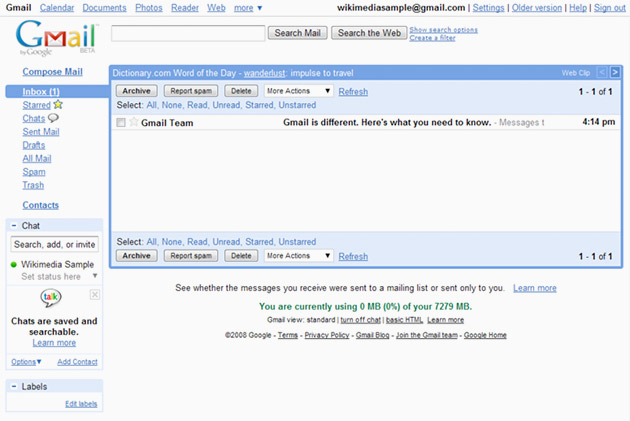
\includegraphics[width=0.4\textwidth]{gmail}
\end{center}

Although the underlying technology hasn't changed much, this interface
provides far more functionality and aligns far better with what businesses
want. Encryption is built-in (when sending internal emails) and users can
send files of any sort (with size restrictions). Users can also organise
their emails and get notifications when they receive a new email --
functionality the old service did not provide. However, it's visually
unappealing. The interface is bland.

\item Third-wave HCI arose as a result of ubiquitous computing. Once everyone
started using computers everywhere, for everything, the focus of UIs was no
longer to maximise functionality but to give users the best experience.
Designers started to come from artistic backgrounds.

Third-wave HCI designs are characterised by pretty, artistic designs
which are often less efficient or provide less functionality than either of
the two previous waves.

\begin{center}
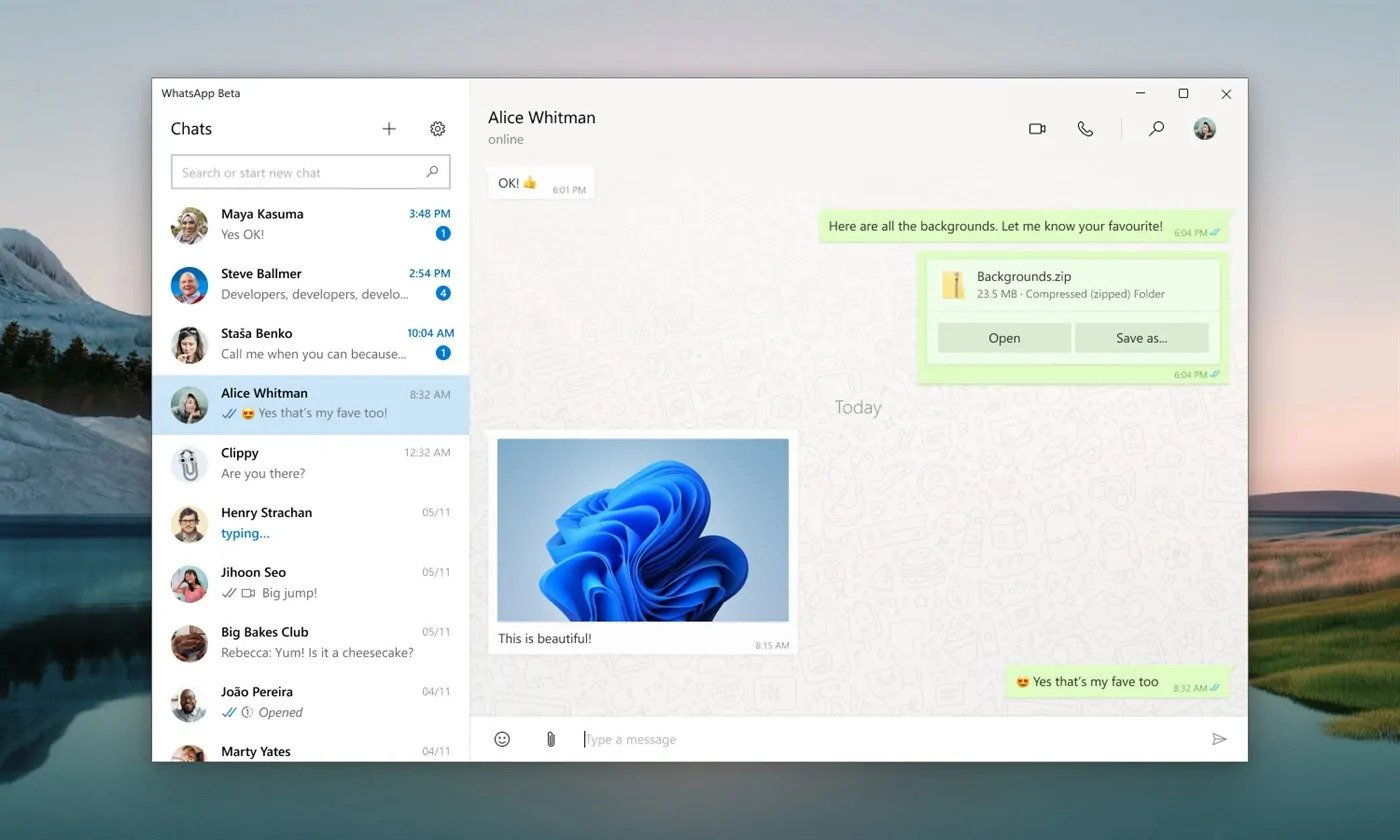
\includegraphics[width=0.4\textwidth]{whatsappjpg}
\end{center}

\item My prediction for fourth-wave HCI is personalisation and customisation.

I believe we are at a first-wave HCI point with visual appeal. In first-wave
HCI, functionality was designed for a specific target user to maximise their
efficiency on very specific tasks. Second-wave HCI realised this model was
wrong and resolved this by ethnography to discover who the \textit{real}
users were and what they \textit{really} wanted.

Third-wave HCI designs interfaces to visually appeal to a specific target
user who wants specific things. As second-wave HCI can attest to (with
regard to functionality), this model is wrong. However UIs work on
internet-scale, so it is infeasible to perform ethnography -- no user
group would be properly represented and many would be completely missed. I
believe the solution to this is high personalisation and customisation
options. Companies have designed their apps and websites to \textit{feel}
how they want them to feel -- or feel how a ``normal'' user would want them
to feel. However, everyone is different -- allowing high customisation
would allow people to feel more comfortable on their own computers and
phones -- an expression of individuality which makes apps better promotes
inclusivity.

The lecturers suggestions about what fourth-wave HCI could involve included
positive computing and accessibility.

I predict that a HCI movement based on accessibility would fail, consider
the case study of Rachael; the American Cancer patient who took on large
companies to get herself on a medicine trial for her cancer; only
\textit{not} to take the medicine (partially) due to the symbolism it
represented. Many people would not turn on accessibility settings because in
doing so, they would admit to themselves they had accessibility needs.

Furthermore, I predict that a HCi movement based on positive computing would
fail -- while the principles are right, the incentives are wrong. Consider
the (widely condemned) 2016 Facebook study into what content users engaged
with. The findings were that users engaged most with negative content. This
is in total contention with the idealistic positive computing HCI revolution.

Personal expression via customisation is a subset of both ideas -- but one
which has no stigma or wrong incentives.

I believe fourth-wave HCI is likely to be characterised by customisable UIs
which allow users to express themselves and \textit{be} themselves --
websites which read system configurations and dynamically create a UI which
reflects the users preferences. We've seen the start of this wave in the
form of support for both dark and light mode.

\end{itemize}

\begin{examquestion}{2018}{7}{6}

\begin{enumerate}

\item Explain in general how the actions that a user takes are related to
the users goals. Your answer should make reference to the function of
perception and to the nature of the cognitive processing that must occur.

There are two main cases.

\begin{itemize}

\item When the user does not know how to achieve their goal.

In this case, the user follows a goal-oriented search. In Computation
Terms, this is a best-first search. The cognitive
processing required is a series of linear scans and a tree traversal of
the UI. A goal-oriented search has four phases:

\begin{itemize}

\item \textbf{Goal}

Formulate what the goal is -- this may be the overall goal ie ``change my
default microphone'' or a smaller sub-goal for example ``open the control
panel''.

\item \textbf{Availability}

The user searches the UI for the best match

\item \textbf{Match}

Once the user has found a match, they click on it.

\item \textbf{Feedback}

The user then sees the results of their action and can evaluate how good a
move it was.

\end{itemize}

However, Goal-Oriented search can fail a number of cases:

\begin{itemize}

\item If the goal is not achievable -- this is a degenerate case. In a
goal-oriented search the user can never actually tell that the goal is not
achievable without enumerating the whole website.

\item If there is a discoverability problem.

In the availability stage, the user searches for the ``best'' match. However,
if there \textit{is} no match then the user cannot choose the ``best'' match.

\item If there is a feedback problem.

In the final stage of goal-oriented search, the user evaluates the success
of the action and considers whether to continue or backtrack. However, if
there \textit{is} no feedback then the user cannot evaluate the success of
the action.

\item Yak Shaving

In some cases, the goal-oriented search will segment the original task into
so many sub-tasks that the user will go on large tangents and forget what the
original task was and what the larger sub-tasks were.

\end{itemize}

\item When the user knows how to achieve their goal

The user knows how to achieve their goals and can proceed without need for a
goal-oriented search. In this case, the user performs the action with
minimal cognitive processing.

If the user has \textit{no muscle memory} and must still search for the
item -- for example when following a guide. Then the time taken to perform
the task can be estimated by Fitts' Law. This forms an expression for the
time required to point to something:
\[
t \propto k \cdot \ln \left( \frac{2 \cdot D}{W} \right)
\]
Where $D$ is the distance to the object and $W$ is the size of the object.
The cognitive processing required is that to point to the correct buttons.

Most humans are satisficers. This means they find a solution which is good
enough and never improve upon it. This means many people who ``know'' how to
perform a task don't know the optimal solution. One part of the theory of
Bounded Rationality is Attention Investment Theory -- this states that
people make decisions not based on the overall outcome, but on how much
time they have to put into it before they get any benefit. Most people will
never learn the most optimal way of doing things even if doing so would
increase their overall utility. For example, most users will spend thousands
of hours on the web -- but never learn shortcuts, instead taking time
(determinable by Fitts' Law) to linearly scan through webpages for
information rather than learning to use \texttt{CTRL-F}.

\end{itemize}

\iffalse

\begin{itemize}

\item Goal-oriented search

\item Satisficing

\item Not rational-choice theory

\item Muscle memory

\item Bounded rationality

\item Fitt's law

\end{itemize}

\fi

\item Describe a class of problems for which it is not possible to formulate
goals. Give a specific example of a problem in this class, and with
reference to that example, explain how it illustrates \textit{two}
significant attributes of the class.

Wicked Problems are a class of (primarily societal and global problems)
which cannot be defined due to contradictory, conflicting or changing
requirements.

The characteristics of a wicked problem are:

\begin{itemize}

\item A Wicked Problem cannot be formulated definitively

\item Wicked problems have no stopping rule

\item Solutions to wicked problems are not true-or-false but good-or-bad

\item Wicked problems have ``one-shot-solutions'' -- there is no opportunity
for trial and error as every attempted solution counts signficantly and
changes the problem

\item Wicked problems do not have an enumerable list of potential solutions

\item Wicked Problems are unique

\item Wicked Problems are symptoms of another problem

\item The cause of discrepancies in wicked problems are open to
interpretation; and the interpretation defines the resolution

\item Planners have no ``right to failure''

\end{itemize}

A classical example of a Wicked Problems is ``solving climate change''.

Consider the problem of solving climate change from the perspective of a
world leader. The world-leader must implement a policy which will ``solve''
climate change. However, it's impossible to evaluate whether or not the
policy works -- the amount by which the planet warms up is continuous --
policies will address climate change to a certain extent. So policies to
solve climate change are ``good'' or ``bad''. If the policy is deemed to
have been ``bad'', then the world leader will be voted out -- therefore they
 have no ``right to failure''.

A more computation example of a Wicked Problem would be ``setting up Linux
without using a guide or wizard''. Enumerating the possible layouts of
files is impossible. You've got one chance to uninstall Windows and install
Linux and if you fail, your computer is permanently damaged and the process
of installing Linux has changed. Once a solution is done, there may be
arbitrary parts of the Linux Kernel which are not set up -- and this may not
be discovered for years.

\item If an interaction system has several alternative models to describe
the user's goal, how can Bayes theorem be used to improve the system usability?

Bayes Theorem is:
\[
\Pr(x\ |\ \overrightarrow{x}) = \frac{\Pr(\overrightarrow{x}\ |\ x) \cdot
\Pr(x)}{\Pr(\overrightarrow{x})}
\]

We could use each of these models to estimate the probability of the users
final goal being $x$ given their inputs $\overrightarrow{x}$. These
probabilities could then be aggregated to form a combined metric estimating
the probability of the users final goal being $x$. The system would order
these and present the user with a sidebar containing several of the most
likely final goals.

Under the ``goal-oriented search'' model, users linearly scan the page until
they find a match for their goal. They then click on it, observe the feedback
and repeat, backtracking where necessary. Systems face usability problems when
there is no match or there is no feedback. By providing suggestions on the
side, we increase the probability of the user finding a match and make
usability failures less likely. If the models describing the users final
goal were sufficiently advanced, they could take account the users
backtracks and failed searches; in this way \textit{every} input
would provide feedback and increase the probability of a match (in the form of
the sidebar changing).

However, this sidebar may appear nondeterminstic from the perspective of a
user. So, while it increases usability for amateur users who perform
goal-oriented search; the sidebar may decrease usability for experienced
users. This could be solved be by adding shortcuts or a ``favourites''
sidebar for experienced users.

\end{enumerate}

\end{examquestion}

\begin{examquestion}{2018}{7}{7}

Imagine that you have been asked to implement a radical new design of your
college website. The Senior Tutor has decided that, to make the college seem
friendlier, the home page and navigation should be implemented using a group
photograph of all members of the college that was taken last summer. Your
task is to design graphical content that will be overlaid onto the
photograph to provide all necessary information and navigation.

\begin{enumerate}

\item Draw a sketch showing the main graphical features of your proposed
design. (A few stick figures will be adequate to represent the original
photograph. No additional marks will be given for realistic depictions of
members of your college.)

\begin{center}
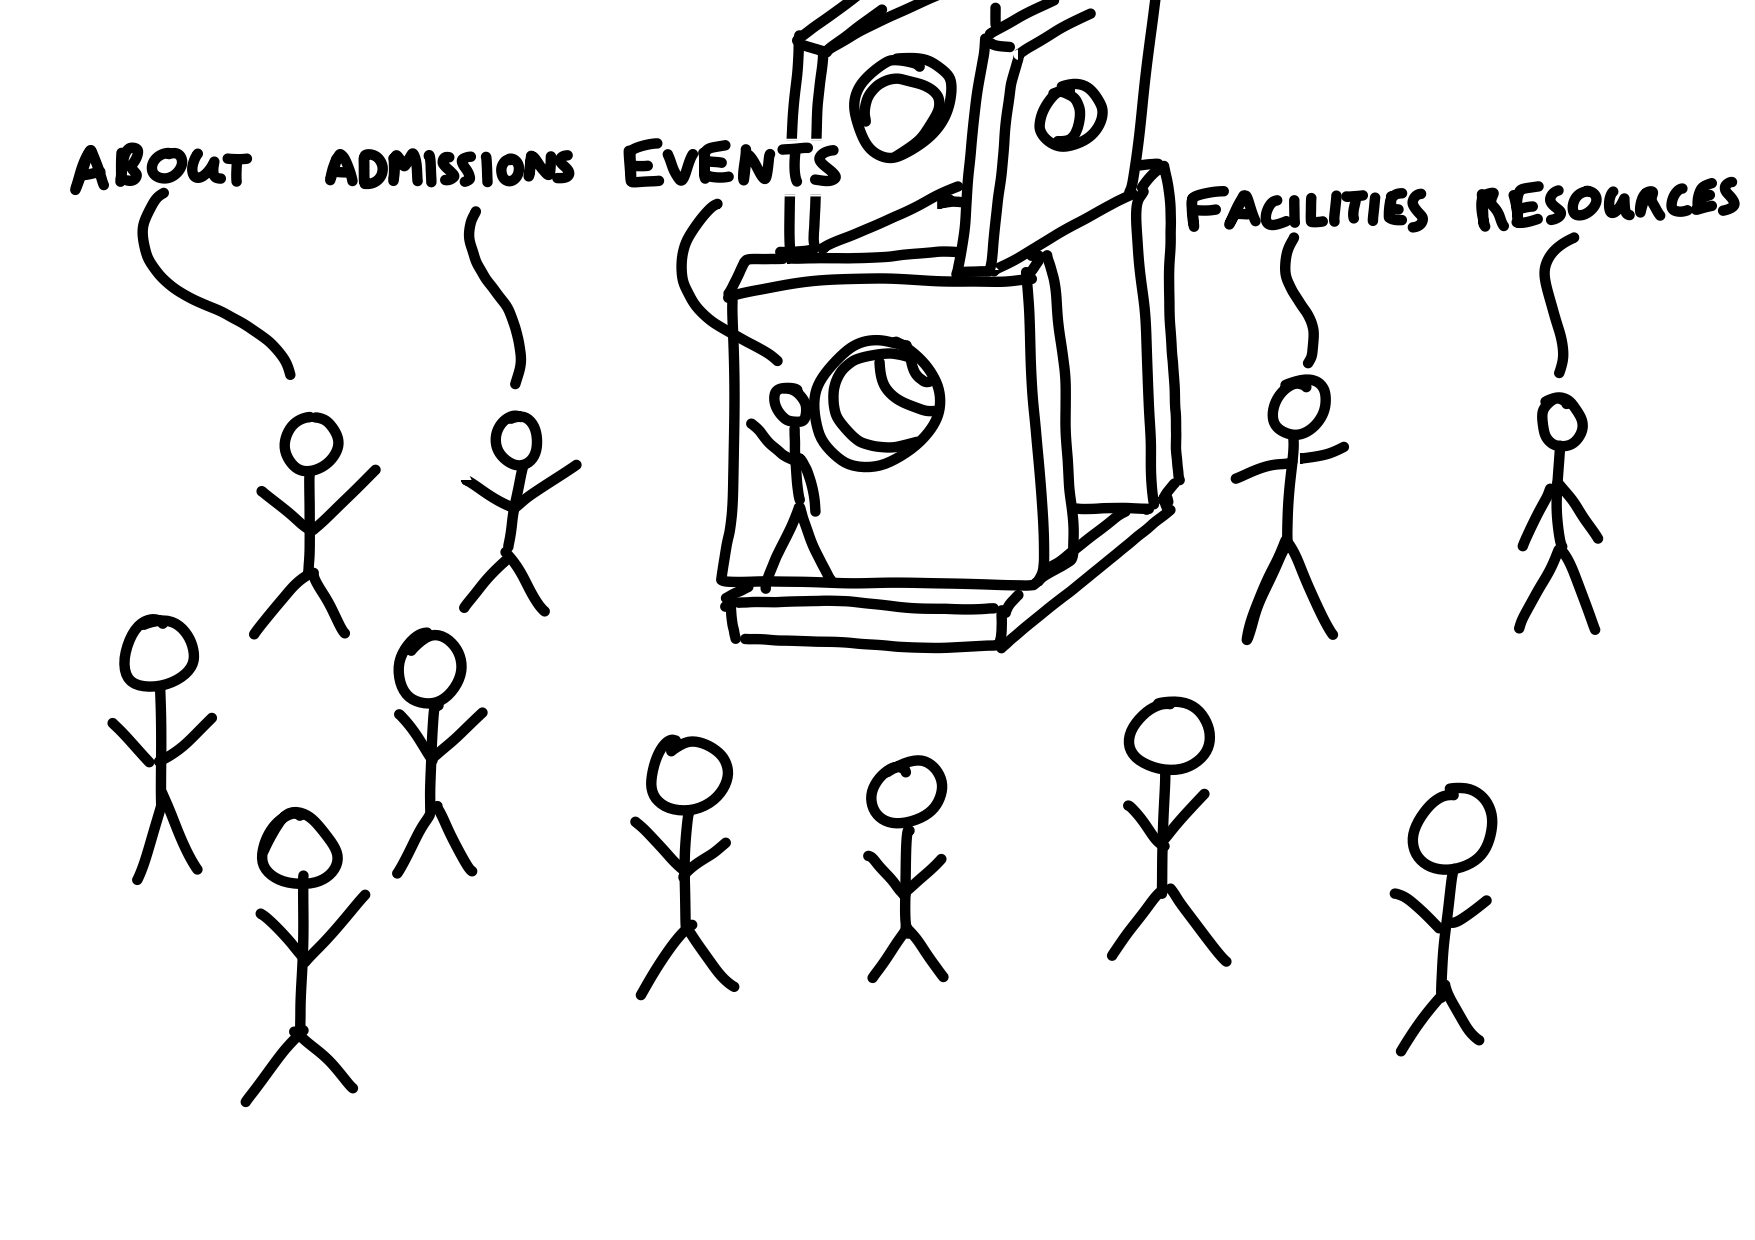
\includegraphics[width=0.8\textwidth]{website_jpg}
\end{center}

\item Explain how the display pane of the photograph has been segmented in
your proposed design, including explanation of any visual marks that were
used to achieve this segmentation.

The design pane of the photograph is naturally segmented in two due to the
sky and the ground. The website design exploits this natural division by
considering the sky to be navigation and the ground to focus on the image --
so as not to obscure the friendly faces of college members. Further
exploitation of the Gestalt Principle of similarity by making all the labels
in the same font helps reinforce to the user that these labels are related
to each other and are distinct from the image. Furthermore, this follows
\textit{existing conventions} and so users are expecting to find headers --
users are used to seeing a natural segmentation between headers and content
and this is exploited.

In many interfaces, text is arranged in a grid-like system. Since the
website is based around an image, it's impossible to enforce a proper grid
without segmenting the image in a visually unappealing way. As a workaround
to this restriction, the webpage uses connecting lines (c.f.\@ node-and-link
diagrams) to connect the faces of the people involved in a particular aspect
of college life to the label linking to the page about that aspect. This
aids in horizontal segmentation of the page.

The whitespace between the labels on the top segments the page -- inspired
by early encyclopedias, this usage of whitespace not to represent a physical
aspect of the college; but as a divider increases usability of the page as
users are naturally divided. Because English is read left-to-right,
top-to-bottom users of the system are likely to perform a linear scan of the
page starting in the top-left. It's therefore essential to ensure the page
is well-segmented and the usage of whitespace aids this.

\item Choose \textit{five} specific visual aspects of your proposed design,
and for \textit{each} of these five:

\begin{enumerate}

\item Describe the graphical property used to implement this aspect (by
reference to your sketch); and

\item Explain the mode of correspondence between this graphical property and
the meaning that is intended in this aspect of your design.

\end{enumerate}

\begin{itemize}

\item Node and Link Diagrams

The primary visual aspect on the design are node-and-link diagrams. Their
usage is a subtle nod towards the technical side of the college (which
could hopefully encourage more applicants). This is intended to connect the
labels to the faces in the image and make the college seem more approachable.

\item Visual metaphor

I've decided to literally connect faces to concepts to help work with the
visual metaphor of ``going up to ask someone about something''. Connecting a
face to a concept will help cement that the college is comprised of real
people and make it less intimidating and more friendly to people considering
applying.

\item Typography and text

An essential part of the website is text -- while metaphor and revolutionary
designs may make the website more appealing and approachable; people
accessing the website will be technically adept and creating a conceptually
new website would greatly decrease usability. Therefore, I've made sure to
layout the labels for concepts across the top -- following
\textit{established conventions} for typography. This will increase
navigability, accessibility and usability.

\item Grid Structure

The main feature which the page relies on for usability is the grid-like
structure -- even though the main focus is on the webpage, and the labels do
not initially appear to be organised (by intentional design), the page
itself is segmented into a grid-like structure. This dramatically increases
usability -- people know where to look for things.

\end{itemize}

\end{enumerate}

\end{examquestion}

\end{document}
